\documentclass[twoside]{book}

% Packages required by doxygen
\usepackage{fixltx2e}
\usepackage{calc}
\usepackage{doxygen}
\usepackage[export]{adjustbox} % also loads graphicx
\usepackage{graphicx}
\usepackage[utf8]{inputenc}
\usepackage{makeidx}
\usepackage{multicol}
\usepackage{multirow}
\PassOptionsToPackage{warn}{textcomp}
\usepackage{textcomp}
\usepackage[nointegrals]{wasysym}
\usepackage[table]{xcolor}

% Font selection
\usepackage[T1]{fontenc}
\usepackage[scaled=.90]{helvet}
\usepackage{courier}
\usepackage{amssymb}
\usepackage{sectsty}
\renewcommand{\familydefault}{\sfdefault}
\allsectionsfont{%
  \fontseries{bc}\selectfont%
  \color{darkgray}%
}
\renewcommand{\DoxyLabelFont}{%
  \fontseries{bc}\selectfont%
  \color{darkgray}%
}
\newcommand{\+}{\discretionary{\mbox{\scriptsize$\hookleftarrow$}}{}{}}

% Page & text layout
\usepackage{geometry}
\geometry{%
  a4paper,%
  top=2.5cm,%
  bottom=2.5cm,%
  left=2.5cm,%
  right=2.5cm%
}
\tolerance=750
\hfuzz=15pt
\hbadness=750
\setlength{\emergencystretch}{15pt}
\setlength{\parindent}{0cm}
\setlength{\parskip}{3ex plus 2ex minus 2ex}
\makeatletter
\renewcommand{\paragraph}{%
  \@startsection{paragraph}{4}{0ex}{-1.0ex}{1.0ex}{%
    \normalfont\normalsize\bfseries\SS@parafont%
  }%
}
\renewcommand{\subparagraph}{%
  \@startsection{subparagraph}{5}{0ex}{-1.0ex}{1.0ex}{%
    \normalfont\normalsize\bfseries\SS@subparafont%
  }%
}
\makeatother

% Headers & footers
\usepackage{fancyhdr}
\pagestyle{fancyplain}
\fancyhead[LE]{\fancyplain{}{\bfseries\thepage}}
\fancyhead[CE]{\fancyplain{}{}}
\fancyhead[RE]{\fancyplain{}{\bfseries\leftmark}}
\fancyhead[LO]{\fancyplain{}{\bfseries\rightmark}}
\fancyhead[CO]{\fancyplain{}{}}
\fancyhead[RO]{\fancyplain{}{\bfseries\thepage}}
\fancyfoot[LE]{\fancyplain{}{}}
\fancyfoot[CE]{\fancyplain{}{}}
\fancyfoot[RE]{\fancyplain{}{\bfseries\scriptsize Generated by Doxygen }}
\fancyfoot[LO]{\fancyplain{}{\bfseries\scriptsize Generated by Doxygen }}
\fancyfoot[CO]{\fancyplain{}{}}
\fancyfoot[RO]{\fancyplain{}{}}
\renewcommand{\footrulewidth}{0.4pt}
\renewcommand{\chaptermark}[1]{%
  \markboth{#1}{}%
}
\renewcommand{\sectionmark}[1]{%
  \markright{\thesection\ #1}%
}

% Indices & bibliography
\usepackage{natbib}
\usepackage[titles]{tocloft}
\setcounter{tocdepth}{3}
\setcounter{secnumdepth}{5}
\makeindex

% Hyperlinks (required, but should be loaded last)
\usepackage{ifpdf}
\ifpdf
  \usepackage[pdftex,pagebackref=true]{hyperref}
\else
  \usepackage[ps2pdf,pagebackref=true]{hyperref}
\fi
\hypersetup{%
  colorlinks=true,%
  linkcolor=blue,%
  citecolor=blue,%
  unicode%
}

% Custom commands
\newcommand{\clearemptydoublepage}{%
  \newpage{\pagestyle{empty}\cleardoublepage}%
}

\usepackage{caption}
\captionsetup{labelsep=space,justification=centering,font={bf},singlelinecheck=off,skip=4pt,position=top}

%===== C O N T E N T S =====

\begin{document}

% Titlepage & ToC
\hypersetup{pageanchor=false,
             bookmarksnumbered=true,
             pdfencoding=unicode
            }
\pagenumbering{alph}
\begin{titlepage}
\vspace*{7cm}
\begin{center}%
{\Large C\+S\+N361\+\_\+\+Assign2 }\\
\vspace*{1cm}
{\large Generated by Doxygen 1.8.13}\\
\end{center}
\end{titlepage}
\clearemptydoublepage
\pagenumbering{roman}
\tableofcontents
\clearemptydoublepage
\pagenumbering{arabic}
\hypersetup{pageanchor=true}

%--- Begin generated contents ---
\chapter{File Index}
\section{File List}
Here is a list of all files with brief descriptions\+:\begin{DoxyCompactList}
\item\contentsline{section}{/media/roodram/72\+F8\+C754\+F8\+C7156\+F/\+Roodram/\+Semester 5/\+Lab/\+Assign2/\hyperlink{_ques1__client_8c}{Ques1\+\_\+client.\+c} }{\pageref{_ques1__client_8c}}{}
\item\contentsline{section}{/media/roodram/72\+F8\+C754\+F8\+C7156\+F/\+Roodram/\+Semester 5/\+Lab/\+Assign2/\hyperlink{_ques1__server_8c}{Ques1\+\_\+server.\+c} }{\pageref{_ques1__server_8c}}{}
\item\contentsline{section}{/media/roodram/72\+F8\+C754\+F8\+C7156\+F/\+Roodram/\+Semester 5/\+Lab/\+Assign2/\hyperlink{_ques2__zombie__orphan_8c}{Ques2\+\_\+zombie\+\_\+orphan.\+c} }{\pageref{_ques2__zombie__orphan_8c}}{}
\end{DoxyCompactList}

\chapter{File Documentation}
\hypertarget{_ques1__client_8c}{}\section{/media/roodram/72\+F8\+C754\+F8\+C7156\+F/\+Roodram/\+Semester 5/\+Lab/\+Assign2/\+Ques1\+\_\+client.c File Reference}
\label{_ques1__client_8c}\index{/media/roodram/72\+F8\+C754\+F8\+C7156\+F/\+Roodram/\+Semester 5/\+Lab/\+Assign2/\+Ques1\+\_\+client.\+c@{/media/roodram/72\+F8\+C754\+F8\+C7156\+F/\+Roodram/\+Semester 5/\+Lab/\+Assign2/\+Ques1\+\_\+client.\+c}}
{\ttfamily \#include $<$stdio.\+h$>$}\newline
{\ttfamily \#include $<$sys/socket.\+h$>$}\newline
{\ttfamily \#include $<$arpa/inet.\+h$>$}\newline
{\ttfamily \#include $<$unistd.\+h$>$}\newline
{\ttfamily \#include $<$string.\+h$>$}\newline
Include dependency graph for Ques1\+\_\+client.\+c\+:
\nopagebreak
\begin{figure}[H]
\begin{center}
\leavevmode
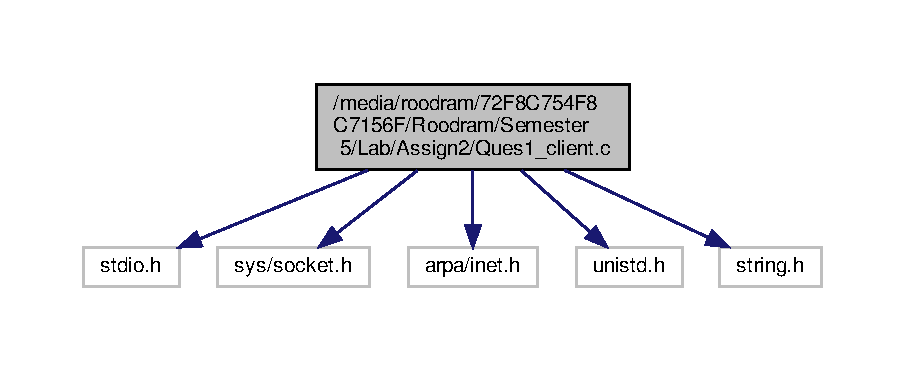
\includegraphics[width=350pt]{_ques1__client_8c__incl}
\end{center}
\end{figure}
\subsection*{Macros}
\begin{DoxyCompactItemize}
\item 
\#define \hyperlink{_ques1__client_8c_a614217d263be1fb1a5f76e2ff7be19a2}{P\+O\+RT}~8080
\end{DoxyCompactItemize}
\subsection*{Functions}
\begin{DoxyCompactItemize}
\item 
int \hyperlink{_ques1__client_8c_abf9e6b7e6f15df4b525a2e7705ba3089}{main} (int argc, char const $\ast$argv\mbox{[}$\,$\mbox{]})
\end{DoxyCompactItemize}


\subsection{Macro Definition Documentation}
\mbox{\Hypertarget{_ques1__client_8c_a614217d263be1fb1a5f76e2ff7be19a2}\label{_ques1__client_8c_a614217d263be1fb1a5f76e2ff7be19a2}} 
\index{Ques1\+\_\+client.\+c@{Ques1\+\_\+client.\+c}!P\+O\+RT@{P\+O\+RT}}
\index{P\+O\+RT@{P\+O\+RT}!Ques1\+\_\+client.\+c@{Ques1\+\_\+client.\+c}}
\subsubsection{\texorpdfstring{P\+O\+RT}{PORT}}
{\footnotesize\ttfamily \#define P\+O\+RT~8080}



\subsection{Function Documentation}
\mbox{\Hypertarget{_ques1__client_8c_abf9e6b7e6f15df4b525a2e7705ba3089}\label{_ques1__client_8c_abf9e6b7e6f15df4b525a2e7705ba3089}} 
\index{Ques1\+\_\+client.\+c@{Ques1\+\_\+client.\+c}!main@{main}}
\index{main@{main}!Ques1\+\_\+client.\+c@{Ques1\+\_\+client.\+c}}
\subsubsection{\texorpdfstring{main()}{main()}}
{\footnotesize\ttfamily int main (\begin{DoxyParamCaption}\item[{int}]{argc,  }\item[{char const $\ast$}]{argv\mbox{[}$\,$\mbox{]} }\end{DoxyParamCaption})}


\hypertarget{_ques1__server_8c}{}\section{/media/roodram/72\+F8\+C754\+F8\+C7156\+F/\+Roodram/\+Semester 5/\+Lab/\+Assign2/\+Ques1\+\_\+server.c File Reference}
\label{_ques1__server_8c}\index{/media/roodram/72\+F8\+C754\+F8\+C7156\+F/\+Roodram/\+Semester 5/\+Lab/\+Assign2/\+Ques1\+\_\+server.\+c@{/media/roodram/72\+F8\+C754\+F8\+C7156\+F/\+Roodram/\+Semester 5/\+Lab/\+Assign2/\+Ques1\+\_\+server.\+c}}
{\ttfamily \#include $<$unistd.\+h$>$}\newline
{\ttfamily \#include $<$stdio.\+h$>$}\newline
{\ttfamily \#include $<$sys/socket.\+h$>$}\newline
{\ttfamily \#include $<$stdlib.\+h$>$}\newline
{\ttfamily \#include $<$netinet/in.\+h$>$}\newline
{\ttfamily \#include $<$string.\+h$>$}\newline
Include dependency graph for Ques1\+\_\+server.\+c\+:
\nopagebreak
\begin{figure}[H]
\begin{center}
\leavevmode
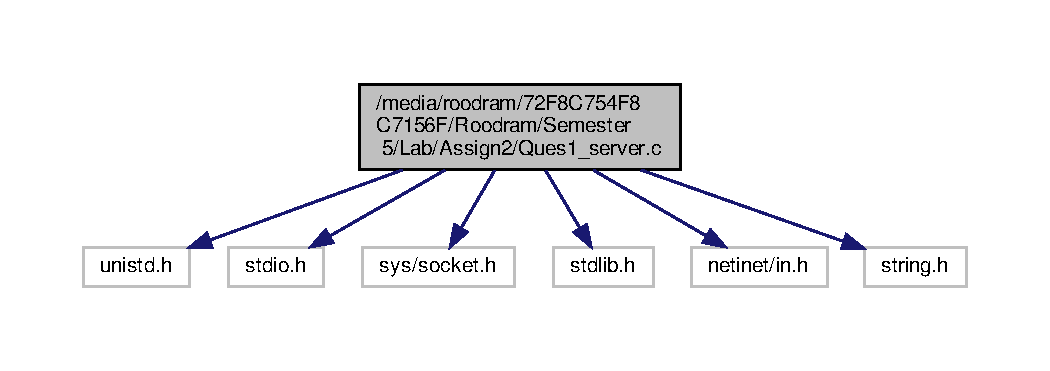
\includegraphics[width=350pt]{_ques1__server_8c__incl}
\end{center}
\end{figure}
\subsection*{Macros}
\begin{DoxyCompactItemize}
\item 
\#define \hyperlink{_ques1__server_8c_a614217d263be1fb1a5f76e2ff7be19a2}{P\+O\+RT}~8080
\end{DoxyCompactItemize}
\subsection*{Functions}
\begin{DoxyCompactItemize}
\item 
int \hyperlink{_ques1__server_8c_abf9e6b7e6f15df4b525a2e7705ba3089}{main} (int argc, char const $\ast$argv\mbox{[}$\,$\mbox{]})
\end{DoxyCompactItemize}


\subsection{Macro Definition Documentation}
\mbox{\Hypertarget{_ques1__server_8c_a614217d263be1fb1a5f76e2ff7be19a2}\label{_ques1__server_8c_a614217d263be1fb1a5f76e2ff7be19a2}} 
\index{Ques1\+\_\+server.\+c@{Ques1\+\_\+server.\+c}!P\+O\+RT@{P\+O\+RT}}
\index{P\+O\+RT@{P\+O\+RT}!Ques1\+\_\+server.\+c@{Ques1\+\_\+server.\+c}}
\subsubsection{\texorpdfstring{P\+O\+RT}{PORT}}
{\footnotesize\ttfamily \#define P\+O\+RT~8080}



\subsection{Function Documentation}
\mbox{\Hypertarget{_ques1__server_8c_abf9e6b7e6f15df4b525a2e7705ba3089}\label{_ques1__server_8c_abf9e6b7e6f15df4b525a2e7705ba3089}} 
\index{Ques1\+\_\+server.\+c@{Ques1\+\_\+server.\+c}!main@{main}}
\index{main@{main}!Ques1\+\_\+server.\+c@{Ques1\+\_\+server.\+c}}
\subsubsection{\texorpdfstring{main()}{main()}}
{\footnotesize\ttfamily int main (\begin{DoxyParamCaption}\item[{int}]{argc,  }\item[{char const $\ast$}]{argv\mbox{[}$\,$\mbox{]} }\end{DoxyParamCaption})}


\hypertarget{_ques2__zombie__orphan_8c}{}\section{/media/roodram/72\+F8\+C754\+F8\+C7156\+F/\+Roodram/\+Semester 5/\+Lab/\+Assign2/\+Ques2\+\_\+zombie\+\_\+orphan.c File Reference}
\label{_ques2__zombie__orphan_8c}\index{/media/roodram/72\+F8\+C754\+F8\+C7156\+F/\+Roodram/\+Semester 5/\+Lab/\+Assign2/\+Ques2\+\_\+zombie\+\_\+orphan.\+c@{/media/roodram/72\+F8\+C754\+F8\+C7156\+F/\+Roodram/\+Semester 5/\+Lab/\+Assign2/\+Ques2\+\_\+zombie\+\_\+orphan.\+c}}
{\ttfamily \#include $<$bits/stdc++.\+h$>$}\newline
{\ttfamily \#include $<$unistd.\+h$>$}\newline
{\ttfamily \#include $<$stdio.\+h$>$}\newline
Include dependency graph for Ques2\+\_\+zombie\+\_\+orphan.\+c\+:
\nopagebreak
\begin{figure}[H]
\begin{center}
\leavevmode
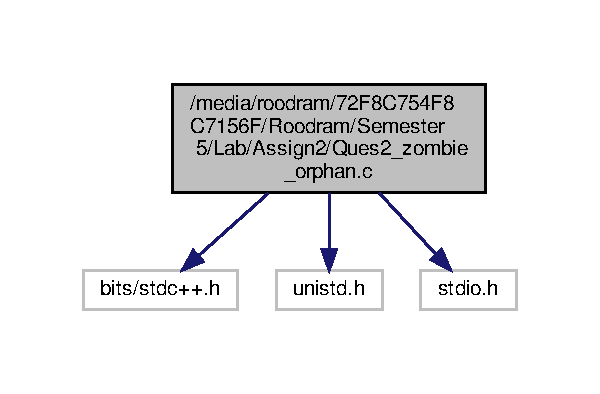
\includegraphics[width=288pt]{_ques2__zombie__orphan_8c__incl}
\end{center}
\end{figure}
\subsection*{Functions}
\begin{DoxyCompactItemize}
\item 
int \hyperlink{_ques2__zombie__orphan_8c_ae66f6b31b5ad750f1fe042a706a4e3d4}{main} ()
\end{DoxyCompactItemize}


\subsection{Function Documentation}
\mbox{\Hypertarget{_ques2__zombie__orphan_8c_ae66f6b31b5ad750f1fe042a706a4e3d4}\label{_ques2__zombie__orphan_8c_ae66f6b31b5ad750f1fe042a706a4e3d4}} 
\index{Ques2\+\_\+zombie\+\_\+orphan.\+c@{Ques2\+\_\+zombie\+\_\+orphan.\+c}!main@{main}}
\index{main@{main}!Ques2\+\_\+zombie\+\_\+orphan.\+c@{Ques2\+\_\+zombie\+\_\+orphan.\+c}}
\subsubsection{\texorpdfstring{main()}{main()}}
{\footnotesize\ttfamily int main (\begin{DoxyParamCaption}{ }\end{DoxyParamCaption})}


%--- End generated contents ---

% Index
\backmatter
\newpage
\phantomsection
\clearemptydoublepage
\addcontentsline{toc}{chapter}{Index}
\printindex

\end{document}
